\documentclass[aspectratio=169,11pt,t]{beamer}
% ============================================================
%  ksa-cs-v2: ksa-cs-lecture-template.tex 스타일 + 한글, v2 덱(16:9)용.
%    - 짙은 네이비 헤드라인 (섹션 이름 + 프레임마다 점)
%    - 꽉 찬 파란 제목 막대, 둥근 그림자 블록
%    - 한글: Noto Sans CJK KR (fontspec)
%  사용:
%    \documentclass[aspectratio=169,11pt,t]{beamer}
%    \input{<..>/theme/ksa-cs-v2.tex}
%  ksa-theme.tex 의 매크로(\kb \kq, ksablue/ksared 등)도 같은 이름으로 둔다
%  -> v2 덱 본문을 거의 그대로 옮길 수 있다.
% ============================================================

\usepackage{fontspec}
\usepackage{amsmath,amssymb}
\usepackage{tikz}
\usepackage{listings}
\usepackage{graphicx}
\usepackage{booktabs}
\usepackage{varwidth}
% enumitem 은 넣지 않는다 (beamer 글머리표가 사라진다)

\defaultfontfeatures{Ligatures=TeX}
\setmainfont{Noto Sans CJK KR}
\setsansfont{Noto Sans CJK KR}
\setmonofont{Noto Sans Mono CJK KR}[Scale=0.92]
\usefonttheme{professionalfonts}

% ---------- 기본 틀 ----------
\usetheme{default}
\useinnertheme[shadow=true]{rounded}
\setbeamertemplate{navigation symbols}{}
\setbeamersize{text margin left=1em,text margin right=1em}

% ---------- 색 (템플릿 원본 값) ----------
\definecolor{navydark}{HTML}{191959}
\definecolor{navydim}{HTML}{8888B0}
\definecolor{navytitle}{HTML}{262686}
\definecolor{navyblue}{HTML}{3333B2}
\definecolor{blockbodybg}{HTML}{E9E9F3}
\definecolor{examplegreen}{HTML}{006000}
\definecolor{examplebg}{HTML}{E5EFE5}
\definecolor{alertred}{HTML}{BF0000}
\definecolor{alertbg}{HTML}{F9E5E5}
% ksa-theme.tex 와 같은 이름 (본문 호환)
\colorlet{ksablue}{navytitle}
\colorlet{ksabluedk}{navydark}
\definecolor{ksagold}{HTML}{D6CBB1}
\definecolor{ksagolddk}{HTML}{A9976B}
\colorlet{ksared}{alertred}
\definecolor{ksagray}{HTML}{5B5B5B}

\setbeamercolor{structure}{fg=navyblue}
\setbeamercolor{alerted text}{fg=alertred}
\setbeamercolor{frametitle}{bg=navytitle,fg=white}
\setbeamercolor{title}{fg=white,bg=navytitle}
\setbeamercolor{block title}{bg=navytitle,fg=white}
\setbeamercolor{block body}{bg=blockbodybg,fg=black}
\setbeamercolor{block title example}{bg=examplegreen,fg=white}
\setbeamercolor{block body example}{bg=examplebg,fg=black}
\setbeamercolor{block title alerted}{bg=alertred,fg=white}
\setbeamercolor{block body alerted}{bg=alertbg,fg=black}
\setbeamercolor{item}{fg=navyblue}
\setbeamertemplate{itemize item}[circle]
\setbeamertemplate{itemize subitem}[triangle]

% ---------- 헤드라인: miniframes (섹션 이름 + 점) ----------
\useoutertheme[subsection=false]{miniframes}
\setbeamerfont{section in head/foot}{size=\tiny}
\setbeamercolor{section in head/foot}{bg=navydark,fg=white}
\setbeamercolor{mini frame}{fg=white}
\setbeamertemplate{mini frames}[circle]

% ---------- 제목 막대: 폭 꽉 채움, 두 줄까지 ----------
\setbeamerfont{frametitle}{size=\normalsize,series=\bfseries}
\setbeamertemplate{frametitle}{%
  \nointerlineskip
  \begin{beamercolorbox}[wd=\paperwidth,ht=2.7ex,dp=1.1ex,leftskip=.3cm,rightskip=.3cm]{frametitle}%
    \usebeamerfont{frametitle}\insertframetitle
  \end{beamercolorbox}}

% ---------- 쪽 번호: 오른쪽 아래 ----------
\setbeamertemplate{footline}{%
  \hfill
  {\color{navydim}\scriptsize\insertframenumber\,/\,\inserttotalframenumber}%
  \hspace{3mm}\vspace{2mm}%
}

% ---------- 표지: 템플릿처럼 헤드라인은 그대로, 가운데 둥근 그림자 상자에 제목 한 줄 ----------
% 덱에서:  {\setbeamertemplate{footline}{}\begin{frame}[c,noframenumbering]\titlepage\end{frame}}
\setbeamercolor{title}{fg=white,bg=navyblue}
\makeatletter
\setbeamertemplate{title page}{%
  \vfill
  \centering
  \begin{minipage}{0.84\paperwidth}
  \begin{beamercolorbox}[wd=\linewidth,sep=7pt,center,rounded=true,shadow=true]{title}
    {\usebeamerfont{title}\inserttitle\par}%
    \ifx\insertsubtitle\@empty\else\vskip0.4em{\usebeamerfont{subtitle}\insertsubtitle\par}\fi
  \end{beamercolorbox}
  \end{minipage}\par\vskip1.6em
  {\usebeamerfont{author}\color{navytitle}\insertauthor\par}\vskip0.3em
  {\usebeamerfont{institute}\color{ksagray}\insertinstitute\par}
  \vfill
}
\makeatother
\setbeamerfont{title}{series=\bfseries,size=\Large}
\setbeamerfont{subtitle}{size=\normalsize}
\setbeamerfont{author}{size=\normalsize}
\setbeamerfont{institute}{size=\small}

% ksa-theme 호환: 덱이 \renewcommand{\ksacredit}{..} 를 해도 되게 (꼬리말에는 안 쓴다)
\newcommand{\ksacredit}{}

% ---------- 강조 ----------
\newcommand{\hl}[1]{\textcolor{alertred}{#1}}
\newcommand{\hlb}[1]{\textcolor{navyblue}{#1}}
\newcommand{\kb}[1]{\textbf{\color{ksablue}#1}}
\newcommand{\kq}[1]{\textbf{\color{ksared}#1}}

% ---------- 파이썬 코드 (템플릿과 같은 색) ----------
\definecolor{codekw}{HTML}{0033B3}
\definecolor{codebuiltin}{HTML}{BF0000}
\definecolor{codestr}{HTML}{067D17}
\definecolor{codecomment}{HTML}{8C8C8C}
\definecolor{codenum}{HTML}{1750EB}
\lstdefinestyle{py}{
  language=Python, basicstyle=\ttfamily\scriptsize,
  keywordstyle=\color{codekw}\bfseries, stringstyle=\color{codestr},
  commentstyle=\color{codecomment}\itshape, numberstyle=\color{codenum},
  emph={print,len,range,sum,input,int,str,float,list,dict,append,remove,sorted,abs,min,max},
  emphstyle=\color{codebuiltin}, showstringspaces=false, keepspaces=true,
  columns=fixed, basewidth=0.52em, aboveskip=1mm, belowskip=1mm, xleftmargin=2mm,
  breaklines=true
}
\lstset{style=py}

% 원본 덱 (ksa-theme): slides/v2/ml1/week05/svm/ -- 그림은 거기 figs/ 를 그대로 쓴다
\setbeamerfont{author}{size=\normalsize}
\setbeamerfont{institute}{size=\small}
\graphicspath{{../../../v2/ml1/week05/svm/figs/}{../../../assets/}}
\makeatletter
\newcommand{\markpage}[1]{\protected@write\@auxout{}{\string\newlabel{#1}{{\the\c@framenumber}{}}}\hypertarget{#1}{}}
\newcommand{\pref}[1]{\hyperlink{#1}{\textcolor{ksagolddk}{(p.\ref{#1})}}}
\makeatother

\renewcommand{\ksacredit}{Machine Learning and Deep Learning \,\textperiodcentered\, 서포트 벡터 머신}
\title{서포트 벡터 머신 (Support Vector Machine)}
\subtitle{가장 넓은 길을 내는 분류기, 그리고 커널 트릭}
\author{Machine Learning and Deep Learning}
\institute{한국과학영재학교 (KSA)}
\date{}
\begin{document}
{\setbeamertemplate{footline}{}\begin{frame}[c,noframenumbering]\titlepage\end{frame}}

\section{질문}
% --- 오늘의 질문
\begin{frame}{오늘의 질문}
\vfill
\begin{columns}[c]
\begin{column}{0.44\textwidth}\centering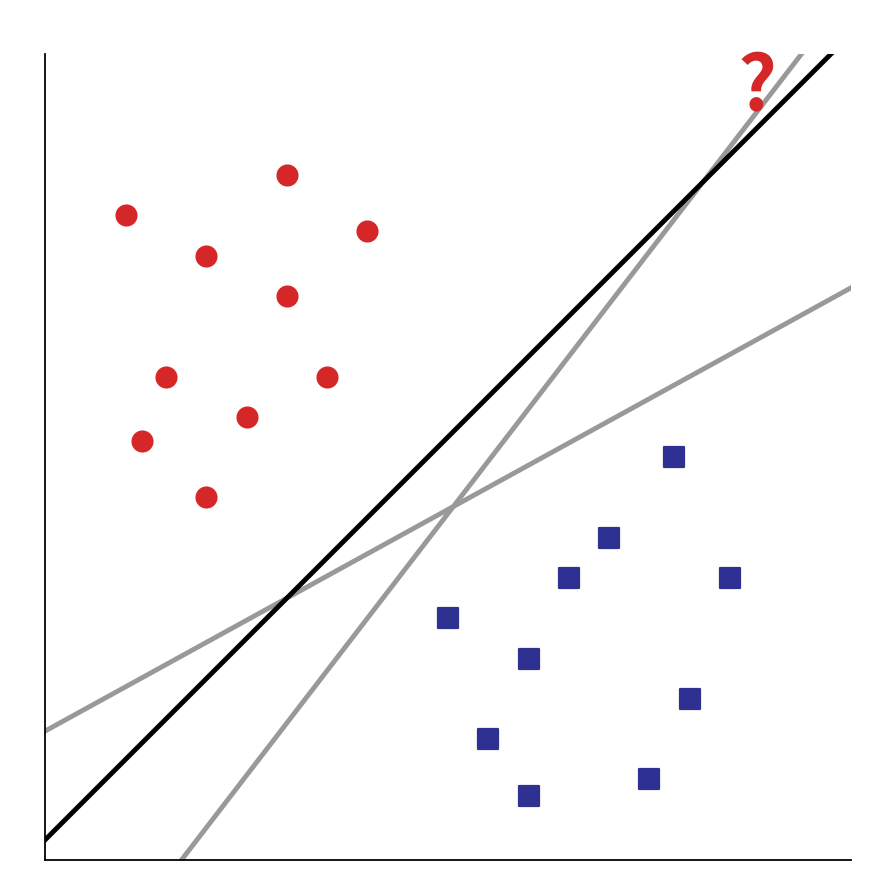
\includegraphics[width=0.95\linewidth]{sv_hook.png}\end{column}
\begin{column}{0.52\textwidth}
{\Large 빨강과 파랑을 가르는 직선}\\[0.8em]
{\large 세 선 모두 학습 데이터를 \textbf{완벽하게} 가른다}\\[0.8em]
{\Large \kq{어느 선이 가장 좋을까?}}
\end{column}
\end{columns}
\vfill
\note{빨간 점과 파란 점이 있습니다. 둘을 가르는 직선을 세 개 그었는데, 세 선 모두 학습 데이터를 하나도 틀리지 않고 완벽하게 가릅니다. 학습 오차로는 셋 다 0입니다. 그런데 어느 선이 가장 좋을까요? 직관적으로는 가운데 검은 선이 가장 안심이 됩니다. 왜 그런지, 그리고 그 선을 어떻게 찾는지가 오늘의 주제입니다.}
\end{frame}

\section{마진}
% --- 바짝 붙은 선
\begin{frame}{점에 바짝 붙은 선은 위험하다}
\vfill
\begin{columns}[c]
\begin{column}{0.44\textwidth}\centering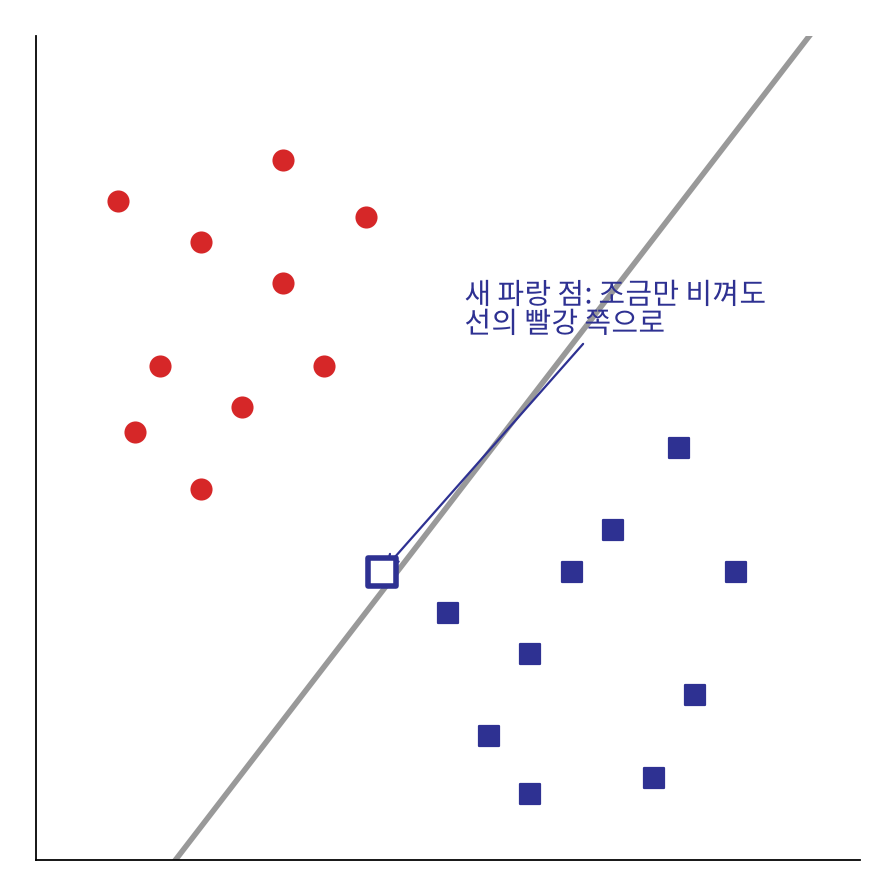
\includegraphics[width=0.95\linewidth]{sv_risky.png}\end{column}
\begin{column}{0.52\textwidth}
{\large 가르는 선은 \textbf{무수히} 많다}\\[0.8em]
{\large 점에 바짝 붙은 선은 새 점이\\ 조금만 비껴 와도 \kq{틀린다}}\\[0.8em]
{\large 양쪽에서 \kb{가장 멀리} 떨어진 선이 안전하다}
\end{column}
\end{columns}
\vfill
\note{가르는 직선은 사실 무수히 많습니다. 그중 파란 점에 바짝 붙은 선을 보세요. 학습 데이터는 맞히지만, 파란 무리 근처에서 새 파란 점이 조금만 위로 비껴 오면 선의 빨강 쪽으로 넘어가서 틀립니다. 측정 오차나 개인차로 새 데이터는 늘 조금씩 비껴 옵니다. 그래서 양쪽 무리에서 가장 멀리 떨어진 선, 양쪽에 여유를 가장 많이 남기는 선이 안전합니다.}
\end{frame}

% --- 가장 넓은 길
\begin{frame}{SVM: 가장 넓은 길을 낸다}
\markpage{street}
\vfill
\begin{columns}[c]
\begin{column}{0.44\textwidth}\centering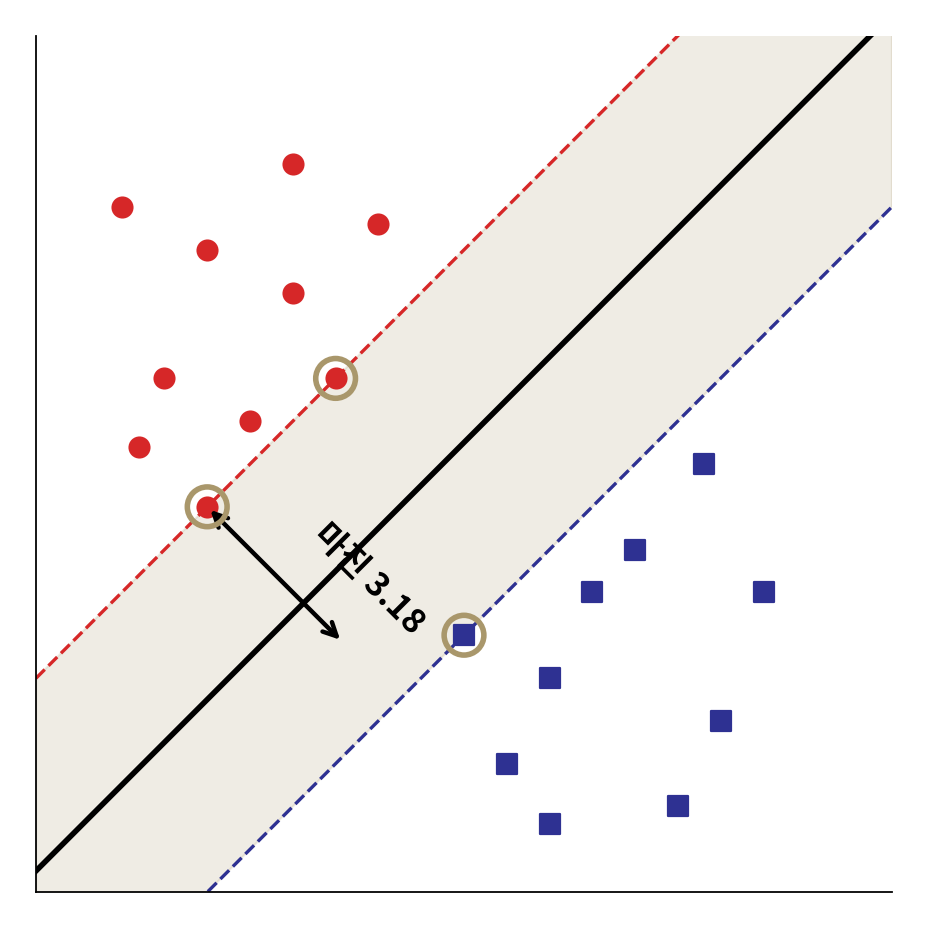
\includegraphics[width=0.95\linewidth]{sv_street.png}\end{column}
\begin{column}{0.52\textwidth}
{\large 두 무리 사이에 \textbf{길}을 낸다}\\[0.6em]
{\large 길의 폭 = \kb{마진 (margin)}}\\[0.6em]
{\large SVM: 마진이 \textbf{가장 넓은} 길의 가운데 선}\\[0.8em]
{\large 이 데이터: 마진 \kb{3.18}}\\[0.4em]
{\small 길 가장자리 (점선) 에 닿은 점 = \textbf{서포트 벡터} (노란 동그라미)}
\end{column}
\end{columns}
\vfill
\note{서포트 벡터 머신, SVM은 두 무리 사이에 길을 냅니다. 길 안에는 점이 하나도 없어야 하고, 길의 폭을 마진이라고 부릅니다. SVM은 마진이 가장 넓은 길을 찾고, 그 길의 가운데 선을 경계로 씁니다. 이 데이터에서 가장 넓은 길의 폭은 3.18입니다. 길 가장자리, 점선에 딱 닿은 점들이 노란 동그라미로 표시돼 있습니다. 이 점들을 서포트 벡터라고 부르고, 이름이 여기서 나왔습니다.}
\end{frame}

% --- 식
\begin{frame}{길을 식으로}
\markpage{form}
\vfill
\centering
{\Large 경계 \quad $\mathbf{w}\cdot\mathbf{x} + b = 0$ \qquad 가장자리 \quad $\mathbf{w}\cdot\mathbf{x} + b = \pm 1$}\\[0.6em]
{\LARGE\[ \min_{\mathbf{w},\,b}\ \frac{1}{2}\lVert\mathbf{w}\rVert^2 \quad \text{subject to} \quad y_i(\mathbf{w}\cdot\mathbf{x}_i + b) \ge 1 \;\; (\text{all } i) \]}\vskip0.2em
\renewcommand{\arraystretch}{1.25}
{\normalsize\begin{tabular}{ll}
$y_i = +1$ (빨강), $-1$ (파랑) & 모든 점이 자기 쪽 가장자리 바깥에 있어야 한다\\
마진 $= 2 / \lVert\mathbf{w}\rVert$ & $\lVert\mathbf{w}\rVert$ 를 줄이면 길이 넓어진다\\
이 데이터 & $\mathbf{w} = \tfrac{4}{9}(-1, 1)$, \; $b = -\tfrac{1}{9}$ \; $\to$ \; $2/\lVert\mathbf{w}\rVert = \tfrac{9}{2\sqrt2} = 3.18$
\end{tabular}}
\vfill
\note{길을 식으로 쓰면 이렇습니다. 경계는 w 점곱 x 더하기 b가 0인 직선, 길 가장자리는 이 값이 플러스 1과 마이너스 1인 직선입니다. 빨강의 라벨을 플러스 1, 파랑을 마이너스 1이라고 하면, 모든 점이 자기 쪽 가장자리 바깥에 있다는 조건은 y 곱하기 w x 더하기 b가 1 이상이라는 한 줄로 쓸 수 있습니다. 두 가장자리 사이의 거리를 계산하면 2 나누기 w의 길이가 나옵니다. 그래서 길을 가장 넓게 하는 것은 w의 길이를 가장 작게 하는 것과 같습니다. 이 데이터에서는 w가 9분의 4 곱하기 마이너스 1, 1이고 b는 마이너스 9분의 1, 마진은 3.18입니다.}
\end{frame}

% --- 서포트 벡터만
\begin{frame}{길 가장자리의 점 몇 개만 선을 정한다}
\vfill
\centering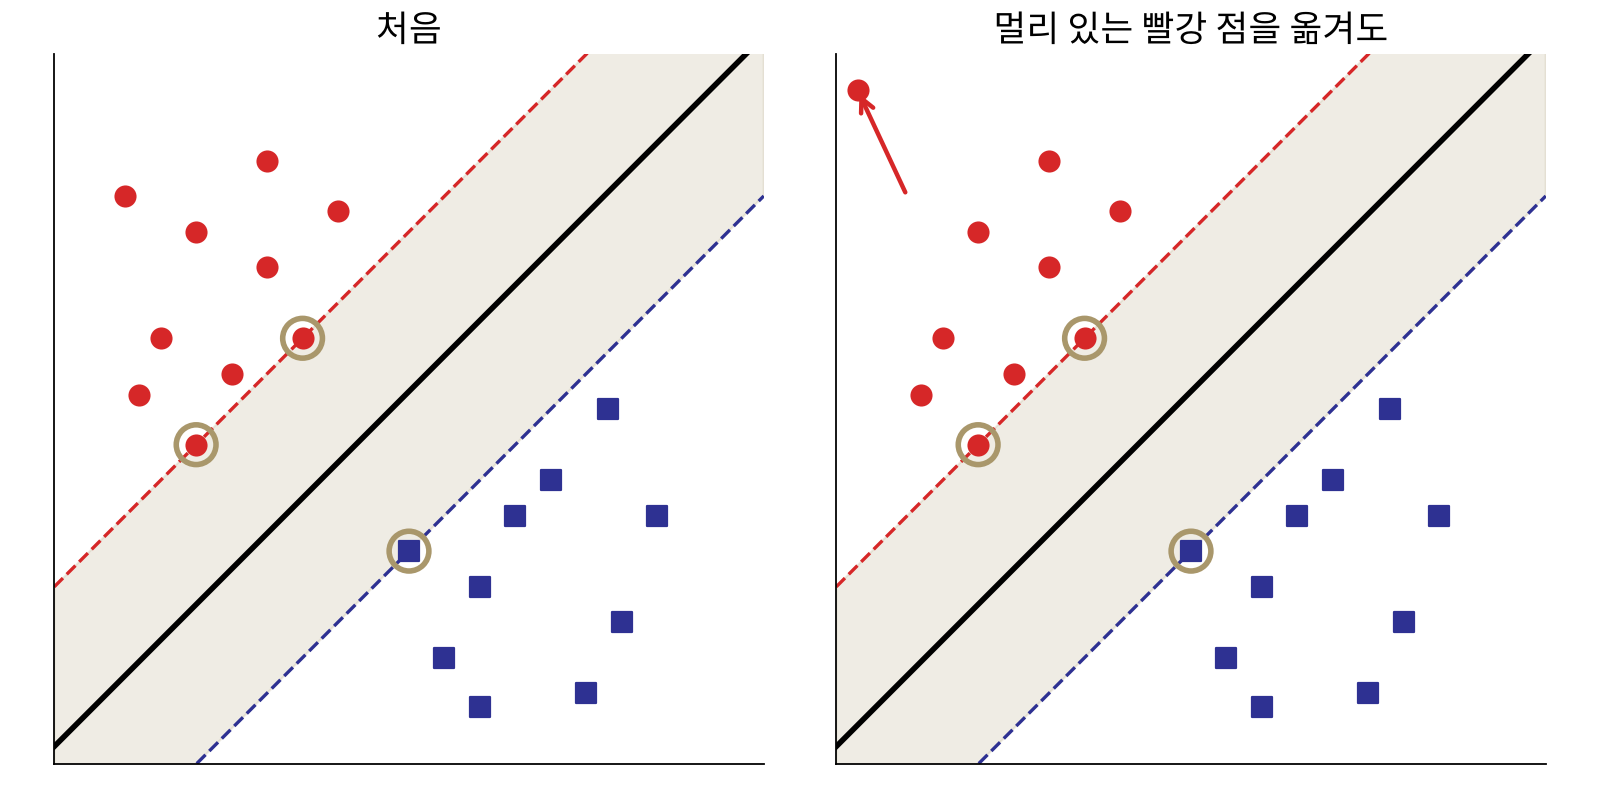
\includegraphics[width=0.66\linewidth]{sv_move.png}\par\vskip0.2em
{\large 서포트 벡터 \kb{3개}: \; $(3.5, 6.0)$, $(2.0, 4.5)$ 빨강 \quad $(5.0, 3.0)$ 파랑}\\[0.2em]
{\large 멀리 있는 점은 옮겨도 경계가 \kq{그대로}}
\vfill
\note{이 경계는 20개 점 중 단 3개, 서포트 벡터가 정합니다. 빨강 둘, 파랑 하나입니다. 길 가장자리에서 멀리 떨어진 점은 경계에 아무 영향이 없습니다. 오른쪽 그림에서 왼쪽 위의 빨간 점 하나를 더 멀리 옮겼는데, 경계와 길은 그대로입니다. 반대로 서포트 벡터 하나를 옮기면 경계가 바뀝니다. 로지스틱회귀는 모든 점이 조금씩 경계에 영향을 주는 것과 대조적입니다.}
\end{frame}

\section{소프트 마진}
% --- 소프트 마진
\begin{frame}{완벽히 나뉘지 않으면: 소프트 마진}
\markpage{soft}
\vfill
\centering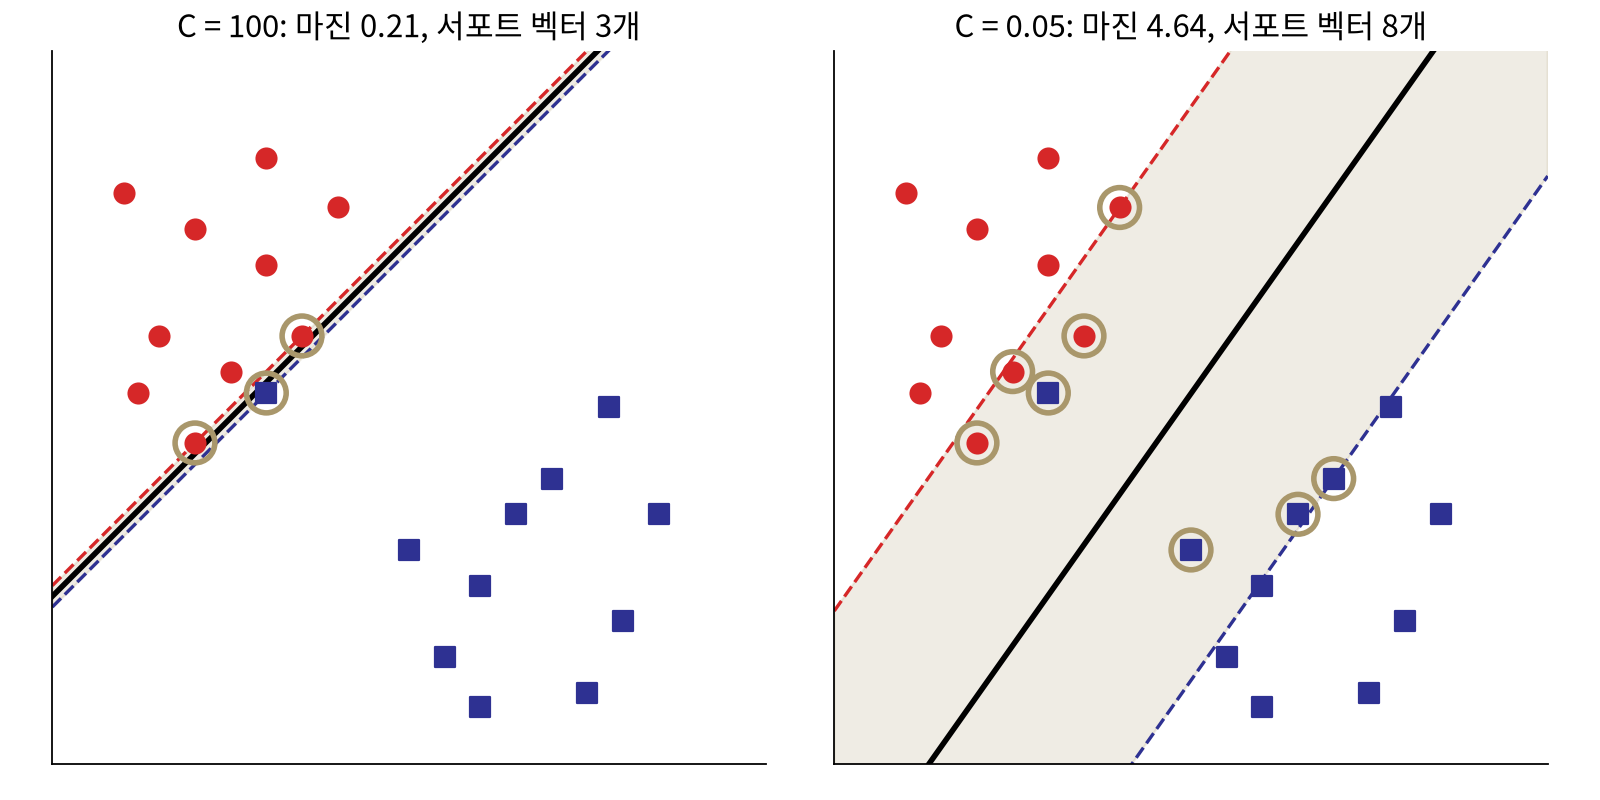
\includegraphics[width=0.53\linewidth]{sv_soft.png}\par\vskip0.1em
{\large\[ \min\ \frac{1}{2}\lVert\mathbf{w}\rVert^2 + \textcolor{ksared}{C}\sum_i \xi_i \qquad \xi_i: \text{가장자리를 넘어간 만큼의 벌점} \]}
{\large $C$ 크면 \kq{안 틀리려고} 좁은 길 (0.21) \quad $C$ 작으면 이상치는 \kb{포기}, 넓은 길 (4.64)}
\vfill
\note{실제 데이터는 이렇게 깔끔하게 나뉘지 않습니다. 빨강 무리 안에 파란 점 하나가 들어왔다고 해 봅시다. 측정 실수일 수도 있습니다. 이러면 길 안에 점이 하나도 없어야 한다는 조건을 지킬 수 없습니다. 그래서 가장자리를 넘어가는 것을 허락하되, 넘어간 만큼 벌점 크사이를 줍니다. C는 그 벌점의 무게입니다. C가 100으로 크면 하나도 틀리지 않으려고 이상치를 피해 가느라 길 폭이 0.21로 아주 좁아집니다. C가 0.05로 작으면 이상치 하나는 틀리기로 하고 4.64짜리 넓은 길을 냅니다. C가 크면 과대적합, 작으면 과소적합 쪽입니다. 그래서 C도 교차 검증으로 고릅니다.}
\end{frame}

\section{커널}
% --- 원 모양 데이터
\begin{frame}{직선으로 못 가르면: 높이를 준다}
\markpage{lift}
\vfill
\centering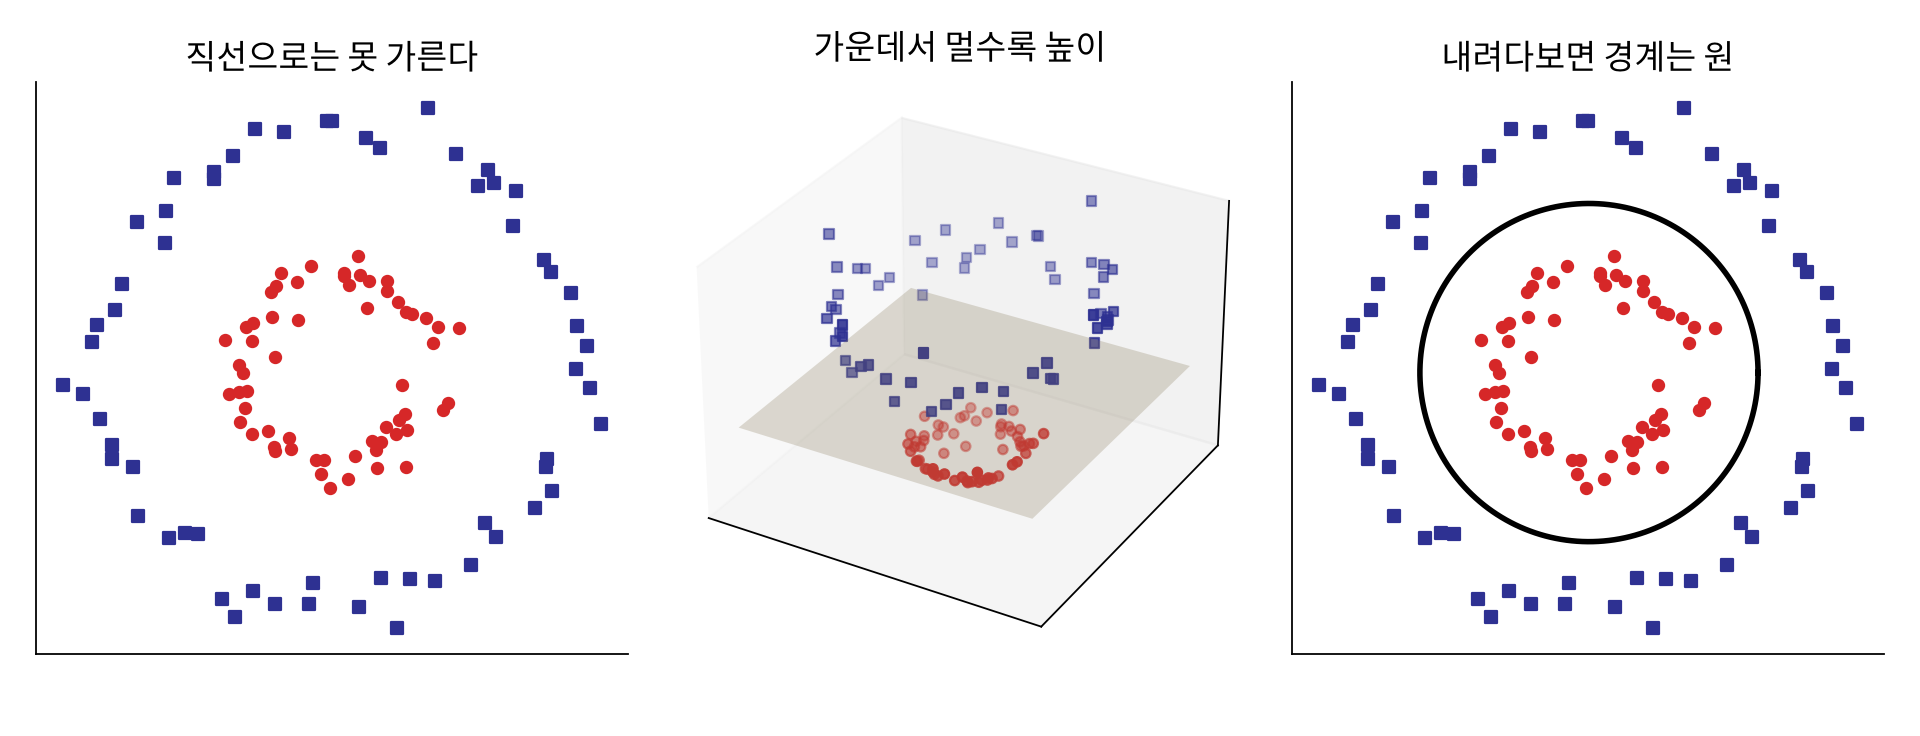
\includegraphics[width=0.94\linewidth]{sv_lift.png}\par\vskip0.2em
{\large 특징 하나를 더한다: \; $(x_1,\ x_2) \;\to\; (x_1,\ x_2,\ \textcolor{ksablue}{x_1^2 + x_2^2})$ \quad $\to$ \quad 평면 하나로 갈라진다}
\vfill
\note{이번에는 빨간 점이 가운데, 파란 점이 바깥을 둘러싼 데이터입니다. 어떤 직선을 그어도 가를 수 없습니다. 그런데 각 점에 높이를 하나 더 줘 봅시다. 가운데서 떨어진 거리의 제곱, x1 제곱 더하기 x2 제곱입니다. 그러면 가운데 빨간 점은 낮게, 바깥 파란 점은 높게 떠서, 가운데 그림처럼 수평한 평면 하나로 깔끔하게 갈라집니다. 이 평면을 원래 평면에서 내려다보면 오른쪽처럼 원이 됩니다. 높은 차원에서 직선으로 가르면, 원래 차원에서는 휘어진 경계가 됩니다. 선형회귀에 x 제곱 특징을 넣은 것과 같은 아이디어입니다.}
\end{frame}

% --- 커널 트릭
\begin{frame}{커널 트릭: 옮기지 않고 계산만}
\markpage{kernel}
\vfill
\centering
{\large SVM 의 계산에는 점끼리의 \textbf{점곱} $\mathbf{x}\cdot\mathbf{x}'$ 만 나온다 $\to$ 점곱 대신 \kb{커널} $K(\mathbf{x},\mathbf{x}')$}\vskip0.4em
{\Large\[ \phi(\mathbf{x}) = (x_1^2,\ \sqrt2\,x_1x_2,\ x_2^2) \quad\Rightarrow\quad \phi(\mathbf{x})\cdot\phi(\mathbf{x}') = (\mathbf{x}\cdot\mathbf{x}')^2 \]}\vskip0.2em
{\large $\mathbf{x} = (1, 2)$, $\mathbf{x}' = (3, 1)$: \quad $(1, 2\sqrt2, 4)\cdot(9, 3\sqrt2, 1) = 9 + 12 + 4 = 25 = (3 + 2)^2$}\\[0.6em]
{\large RBF 커널 \; $K(\mathbf{x},\mathbf{x}') = \exp\!\big(-\gamma\lVert\mathbf{x}-\mathbf{x}'\rVert^2\big)$ \; = 무한 차원으로 옮긴 것과 같다}
\vfill
\note{높은 차원으로 옮기면 특징이 많아져 계산이 무거워집니다. 그런데 SVM을 풀 때는 점 자체가 아니라 점끼리의 점곱만 필요하다는 게 알려져 있습니다. 그래서 옮긴 뒤의 점곱을 옮기지 않고 바로 계산하는 함수, 커널을 씁니다. 예를 들어 2차원 점을 x1 제곱, 루트2 x1 x2, x2 제곱인 3차원으로 옮기면, 옮긴 뒤의 점곱은 원래 점곱의 제곱과 정확히 같습니다. (1, 2)와 (3, 1)이면 옮겨서 계산해도 25, 원래 점곱 5를 제곱해도 25입니다. 이렇게 옮기지 않고 계산만 하는 요령이 커널 트릭입니다. 가장 많이 쓰는 RBF 커널은 무한 차원으로 옮긴 것과 같은 효과를 내는데도 계산은 거리 하나면 됩니다.}
\end{frame}

% --- gamma
\begin{frame}{RBF 커널의 $\gamma$: 얼마나 구불구불하게}
\vfill
\centering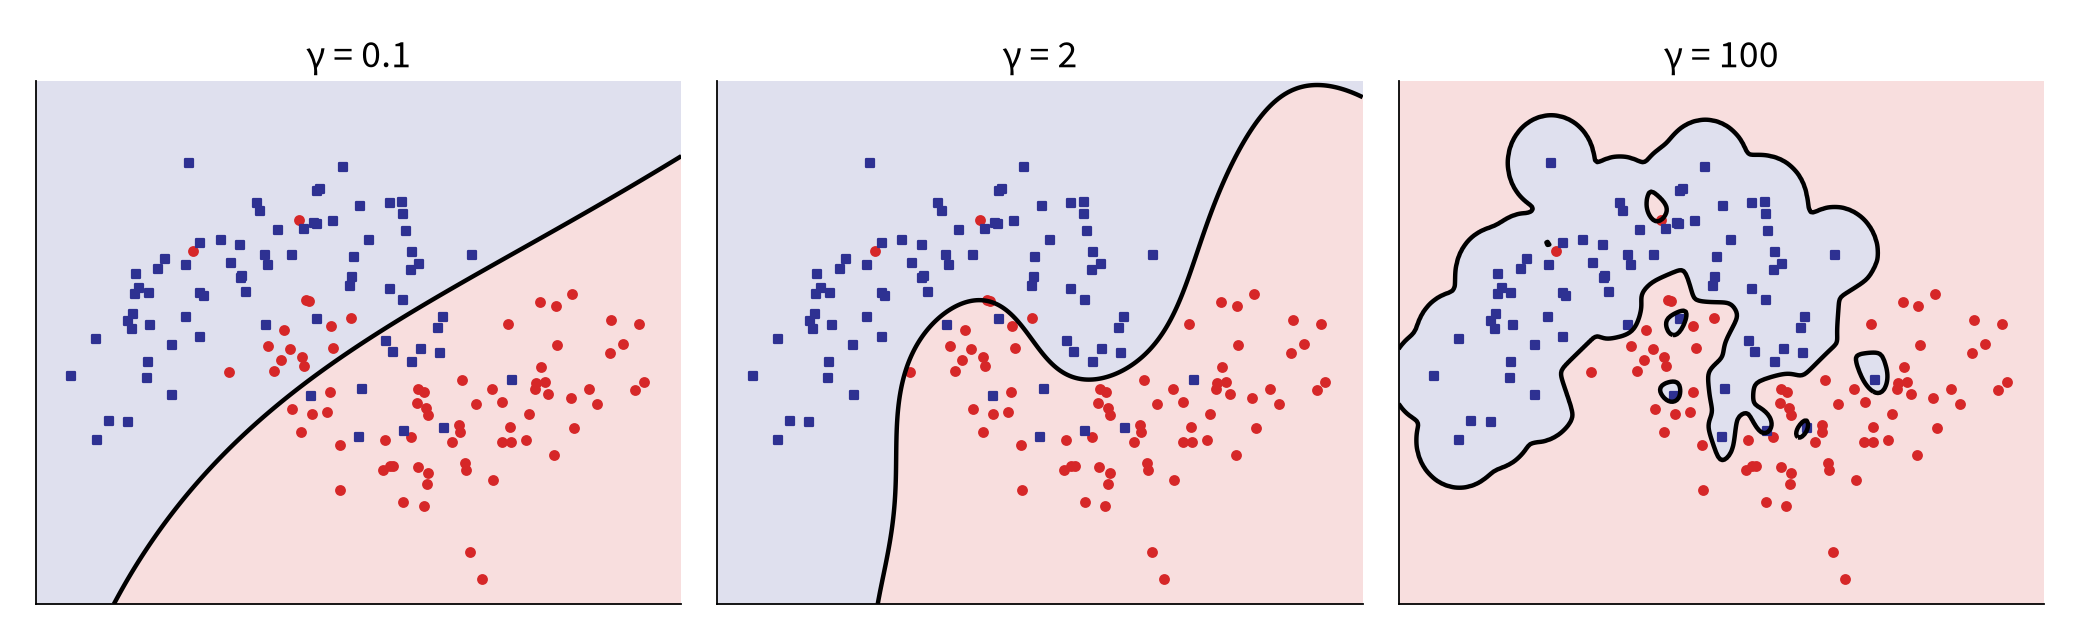
\includegraphics[width=0.92\linewidth]{sv_gamma.png}\par\vskip0.2em
{\large $\gamma$ 작으면 거의 직선 (과소적합) \quad $\gamma$ 크면 점마다 섬 (\kq{과대적합}) \quad $\to$ $C$, $\gamma$ 는 교차 검증으로}
\vfill
\note{RBF 커널의 감마는 점 하나의 영향이 얼마나 멀리까지 미치는지를 정합니다. 감마가 0.1로 작으면 영향이 넓게 퍼져서 경계가 거의 직선입니다. 반달 모양을 못 따라가는 과소적합입니다. 감마가 2면 반달을 따라 적당히 휘어집니다. 감마가 100이면 점 하나하나의 영향이 아주 좁아서 점마다 섬이 생깁니다. 학습 데이터를 외운 과대적합입니다. 그래서 SVM을 쓸 때는 C와 감마 두 숫자를 교차 검증으로 함께 고릅니다. 실습에서 직접 해 봅니다.}
\end{frame}

\section{연습}
% --- 문제풀이
\begin{frame}{문제풀이}
\vfill
\begin{enumerate}
\item 1차원 점: 빨강 $x = 4, 5$, 파랑 $x = 1, 2$. (a) 가장 넓은 길의 경계와 마진은? \; (b) 서포트 벡터는?\vskip0.8em
\item $\mathbf{w} = (3, 4)$ 인 SVM 의 마진은?\vskip0.8em
\item 학습 정확도 100\%, 검증 정확도 70\% 인 RBF SVM. $C$ 와 $\gamma$ 를 어느 쪽으로 바꿔 보겠나?\vskip0.8em
\item $\mathbf{x} = (2, 0)$, $\mathbf{x}' = (1, 3)$ 일 때 $(\mathbf{x}\cdot\mathbf{x}')^2$ 와 $\phi(\mathbf{x})\cdot\phi(\mathbf{x}')$ 를 각각 계산해 같은지 확인하라.
\end{enumerate}
\vfill
\note{1번 답. 가장 가까운 두 점이 2와 4이니 경계는 가운데 3, 마진은 2입니다. 서포트 벡터는 2와 4입니다. 2번 답. w의 길이가 5이니 마진은 2 나누기 5, 0.4입니다. 3번 답. 과대적합이니 C와 감마를 둘 다 줄여 봅니다. 4번 답. 점곱이 2라서 제곱하면 4입니다. 파이 x는 (4, 0, 0), 파이 x 프라임은 (1, 3루트2, 9)이니 점곱은 4, 같습니다.}
\end{frame}

% --- 실습
\begin{frame}{실습}
\vfill
\centering\begin{tabular}{rl}
\large 1 & 슬라이드의 점 20개로 선형 SVM: 마진 3.18, 서포트 벡터 3개, 먼 점 옮기기 재현\\[0.5em]
\large 2 & 실제 데이터: 지폐 1,372장 진위 판별, 선형 vs RBF\\[0.5em]
\large 3 & 원 · 반달 데이터에서 $C$ 와 $\gamma$ 를 교차 검증으로 고르기
\end{tabular}\vskip1em
Banknote Authentication (Lohweg; UCI) \\[0.4em]\href{https://colab.research.google.com/github/SuminHan/book-ml/blob/main/slides/v2/ml1/week05/svm/lab/svm.ipynb}{\textcolor{ksagolddk}{▶ Colab에서 실습 노트북 열기}}
\vfill
\note{실습은 세 부분입니다. 첫째, 슬라이드의 점 20개로 선형 SVM을 학습해서 마진 3.18과 서포트 벡터 3개를 재현하고, 먼 점을 옮겨도 경계가 그대로인지 확인합니다. 둘째, 지폐 사진에서 뽑은 특징 4개로 진짜 지폐와 위조지폐를 가리는 실제 데이터에서 선형 SVM과 RBF SVM을 비교합니다. 셋째, 원과 반달 데이터에서 C와 감마를 교차 검증으로 고르고 경계를 그려 봅니다.}
\end{frame}

\section{정리}
% --- 정리
\begin{frame}{정리}
\vfill
\centering\large\begin{tabular}{l}
\textbf{SVM} \quad 마진 (길의 폭) 이 가장 넓은 경계 \quad $\min \frac12\lVert\mathbf{w}\rVert^2$\\[0.5em]
경계는 길 가장자리의 \kb{서포트 벡터} 몇 개가 정한다\\[0.5em]
\textbf{소프트 마진} $C$: 크면 좁은 길 (과대적합), 작으면 넓은 길\\[0.5em]
\textbf{커널 트릭}: 옮기지 않고 높은 차원의 점곱 $\to$ 휘어진 경계 (RBF 의 $\gamma$)
\end{tabular}
\vfill
\note{정리합니다. SVM은 마진, 즉 길의 폭이 가장 넓은 경계를 찾고, 식으로는 w의 길이 제곱을 최소화하는 문제입니다. 경계는 길 가장자리의 서포트 벡터 몇 개가 정하고, 나머지 점은 영향이 없습니다. 깔끔하게 나뉘지 않으면 소프트 마진을 쓰고, C가 크면 좁은 길로 과대적합, 작으면 넓은 길로 과소적합 쪽입니다. 직선으로 안 되면 커널 트릭으로 높은 차원의 점곱을 바로 계산해서 휘어진 경계를 만들고, RBF 커널의 감마로 얼마나 휠지 정합니다.}
\end{frame}
\end{document}
